\documentclass[8pt,a4paper,compress,handout]{beamer}

\usepackage{/home/siyer/lib/slides}

\title{PicoBot}
\date{}

\begin{document}
\begin{frame}
\begin{flushright}
\tiny \textsc{I ache, therefore I am. \\ - Marvin, the Paranoid Android from The Hitchhiker's Guide to the Galaxy}
\end{flushright}
\titlepage
\end{frame}

\begin{frame}
\frametitle{Outline}
\tableofcontents
\end{frame}

\section{The Roomba Problem}
\begin{frame}[fragile]
PicoBot is a simple programming language that controls a robot (also referred to as PicoBot) loosely based on the Roomba vacuum cleaner robot.

\bigskip

PicoBot's goal is to suck up the debris from the free space around it, ideally without missing any nooks or crannies; the robotics community refers to this as the \emph{coverage problem}.

\bigskip

PicoBot's limitations:
\begin{itemize}
\item it can only sense what's directly around it; 

\item it is totally unfamiliar with the environment it is supposed to clean; and 

\item it can't remember which part of the room it has seen and which part it has not.
\end{itemize}

\bigskip

Simulation environments for exploring PicoBot's capabilities:
\begin{itemize}
\item \href{http://www.cs.hmc.edu/picobot/}{http://www.cs.hmc.edu/picobot/} (online)

\item \href{https://github.com/swamiiyer/picobot.git}{https://github.com/swamiiyer/picobot.git} (command-line)
\end{itemize}
\end{frame}

\section{The Environment}
\begin{frame}[fragile]
\begin{minipage}{200pt}
We will model the environment, i.e., the room a PicoBot is supposed to clean, as a two-dimensional plane discretized into cells.

\bigskip

The cells are either green (PicoBot itself), blue (obstacle or wall), dark gray (visited), or light gray (unvisited). 

\bigskip

PicoBot can't sense whether an empty cell has been visited or not, but it can sense whether each of its four immediate neighbors is free space or an obstacle.

\bigskip

The immediate surroundings of a PicoBot are reported as a string of four letters in \lstinline{NEWS} order.

\bigskip

If the cell in a particular direction is not occupied (i.e., not an obstacle), then the letter in the corresponding position is an \lstinline{x} (or \lstinline{X}). 

\bigskip

For example, at its position in the lower-left-hand corner of the environment shown, the PicoBot's sensors would report its surroundings as \lstinline{xxWS}.
\end{minipage}\hfill%
\begin{minipage}{100pt}
\begin{center}
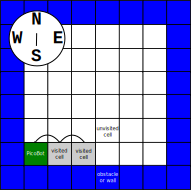
\includegraphics[scale=0.25]{figures/picobot_env.png}

\smallskip

\tiny PicoBot environment

\smallskip

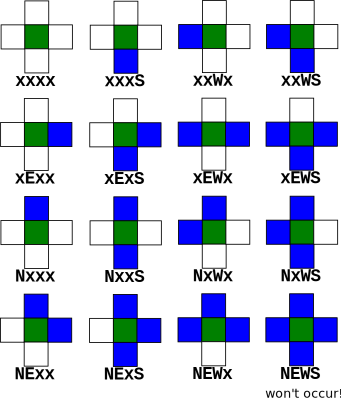
\includegraphics[scale=0.25]{figures/picobot_surroundings.png}

\smallskip

\tiny Possible surrounding strings for PicoBot
\end{center}
\end{minipage}
\end{frame}

\section{State}
\begin{frame}[fragile]
The \emph{state} of a computer is the internal information that describes what the computer is doing.

\bigskip

PicoBot's state is simply a number (0-99) representing a task that you would like PicoBot to undertake.

\bigskip

PicoBot always starts in state 0.
\end{frame}

\section{Rule}
\begin{frame}[fragile]
PicoBot moves by following a set of rules that specify actions and possibly state changes. 

\bigskip

Which rule PicoBot chooses to follow depends on its current state and its current surroundings.

\bigskip
Each PicoBot rule has a five-part syntax:
\begin{lstlisting}[language={}]
<current state> <surrounding string> -> <action> <new state>
\end{lstlisting}
where \lstinline{<action>} is \lstinline{N} (move north), \lstinline{E} (move east), \lstinline{W} (move west), \lstinline{S} (move south), or \lstinline{x}/\lstinline{X} (stay put).

\bigskip

The \lstinline{<surrounding string>} in a PicoBot rule may include wildcards (\lstinline{*}), meaning the PicoBot doesn't care about the surroundings in the corresponding positions.

\bigskip

Examples:
\begin{itemize}
\item \lstinline{0 xxWx -> E 1} $\implies$ ``If I'm in state 0 and only my western neighbor contains an obstacle, take one step east and change into state 1.''

\item \lstinline{0 xxxx -> W 0} $\implies$ ``If I'm in state 0 with no obstacles around me, move one step west and stay in state 0.''
\end{itemize}
\end{frame}

\section{Algorithm}
\begin{frame}[fragile]
An algorithm (in English) instructing a PicoBot to move back and forth in an empty room:
\begin{enumerate}
\item Move west until PicoBot hits a wall to the west.

\item Then move east until PicoBot hits a wall to the east.

\item Then go back to step 1.
\end{enumerate}

\bigskip

The above algorithm in PicoBot:
\begin{lstlisting}[language={}]
0 **x* -> W 0

0 **W* -> E 1

1 *x** -> E 1

1 *E** -> W 0
\end{lstlisting}
\end{frame}

\section{Uncomputable Environments}
\begin{frame}[fragile]
It can be shown mathematically that PicoBot's computational capabilities aren't enough to guarantee coverage of all environments.

\bigskip

By adding one simple feature to PicoBot --- the ability to drop, sense, and pick up ``markers'' along the way --- it can be programmed to fully explore any environment. 

\bigskip

It is true in general that certain problems are beyond the limits of what computers can solve.
\end{frame}
\end{document}
